\chapter{Introduction}
\label{chap:intro}

This chapter gives a general introduction to the subject. First, the problem with 
classic terrestrial networks is explained and illustrated with some examples. Thereafter, 
the research questions that are believed to give a solution to this problem are discussed.
Finally, an overview of the entire document is given.

\section{Outline of the Issue} %1p
\label{sec:issue}

% inspiratie kan je hier ook nog vinden:
% PREDICTION AND COMPARISON OF DOWNLINK ELECTRICFIELDAND UPLINK LOCALISED SARVALUES FOR REALISTIC INDOOR WIRELESS PLANNING
Society is constantly getting more and more dependent on wireless communication. 
On any given moment, in any given location, an electronic device
can request to connect to the bigger network. Devices need more than ever to be connected, 
starting from small \gls{IOT} up to self-driving cars
which all need to be supported by the existing infrastructure. 
It is not surprising that the city centre of Ghent has an average coverage of 97\% of 4G over all telecom operators
\cite{testaankoop}. Once again it becomes clear why we're on the eve of a new generation of cellular communication named 5G. 

Also in exceptional and possibly life-threatening situations, the public relies on the cellular network. 
In 2011, Pukkelpop, a yearly festival in Belgium, got struck by a severe storm. However the storm 
was quite short, the damage was done, including the mobile network which remained defective for the rest of the evening \cite{pukkelpop}.
One solution for a fast temporarily deployable network is with the usage of \gls{UAV}s. Base stations can be attached to 
these flying \gls{UAV}s to support the damaged network over a limited area. 
This approach does not only come in handy for 
damaged networks but also in case of an unexpected increase of traffic. 
For example during the terrorist attacks at Brussels Airport,
mobile network operators saw all telecommunications drastically increasing causing moments of contention. 
Some operators even decided to temporarily exceed the exposure limits in
order to handle all connections \cite{baseZaventem}.
This is illustrated in figure \ref{fig:networkIllustrationDamagedNetwork}.
Electromagnetic exposure can however not be neglected. Research shows how excessive electromagnetic radiation can cause diverse biological side effects \cite{J31_bioeffects}.
Because of increasing public concern \cite{J31_bioeffects}, the \gls{WHO} had launched a large multidisciplinary research effort which eventually concluded that there was no sufficient evidence that confirmed 
that exposure to low level electromagnetic fields is harmful \cite{WHO}. 
A large part of the population remains nevertheless very concerned about potential health risks \cite{bloomberg5G}.
It becomes clear that electromagnetic exposure is a key value when designing a \gls{UAV}-aided network and should definitely 
not surpass the predefined limits.

\begin{figure}[H]
\centering
  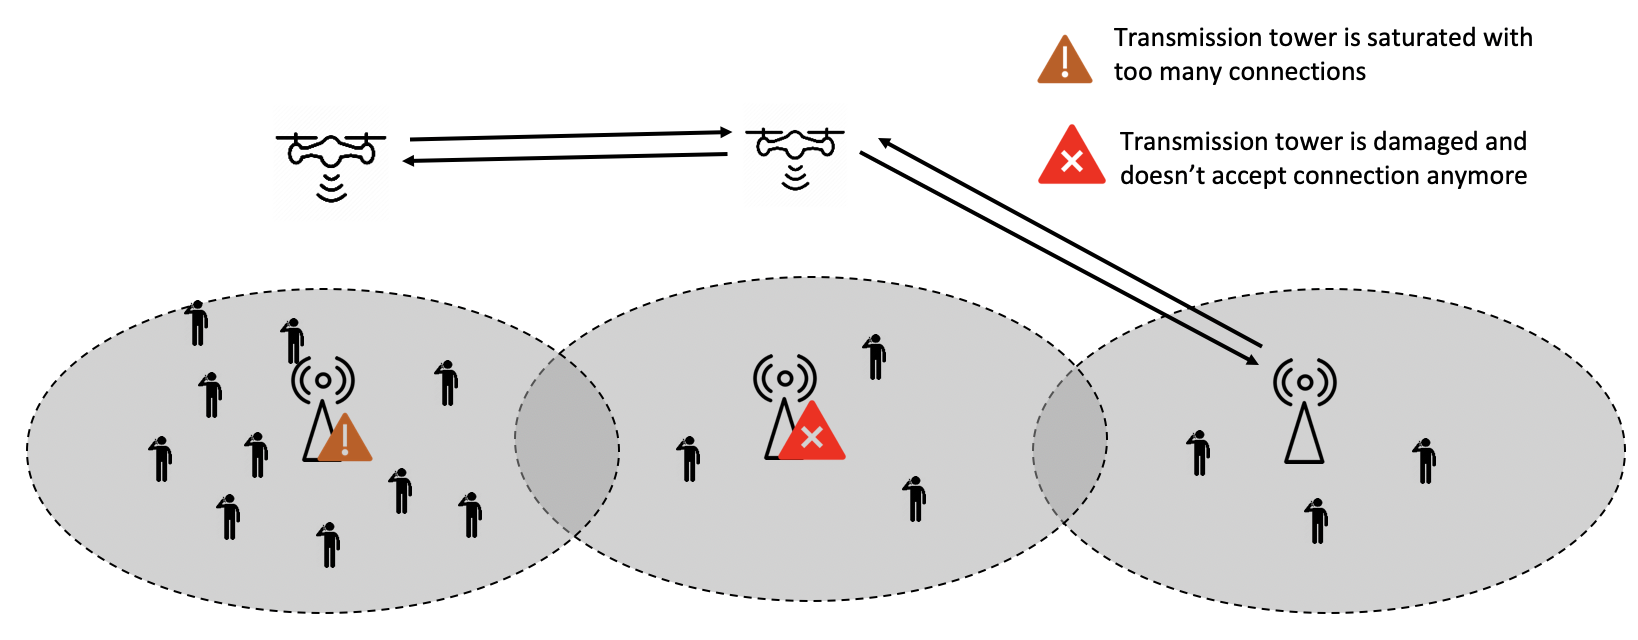
\includegraphics[width=\textwidth]{../images/networkIllustrationDamagedNetwork.png}
  \caption{This illustration shows how a UAV-aided network is able to either assist or replace 
  existing transmission towers.}
  \label{fig:networkIllustrationDamagedNetwork}
\end{figure}

\section{Objective}
\label{sec:objective}

\gls{UAV}-aided networks can, thanks to their mobility, easily be repositioned towards a certain goal. Several papers 
in literature exist, explaining how a network can be optimized towards different goals like power consumption.
However, very limited
research has been done where a \gls{UAV}-aided network is optimized towards electromagnetic exposure.
While several publications exist, discussing how the electromagnetic exposure can be calculated, most of them only consider a limited number of sources like only base stations or only mobile phones.
Papers who cover electromagnetic exposure from all the different sources and convert it into a single value are rather limited.

This master dissertation proposes a method to optimize the network towards electromagnetic exposure and power consumption
when considering all four sources of radiation in a telecommunications network, being: the user's own phone, 
the base station that is serving this user, 
all devices from other users in the network and all 
other active base stations that are not serving this user. In this way, the contribution of each source towards the total 
electromagnetic exposure can easily be identified. 

The behaviour of the electromagnetic exposure and power consumption of the network will be analysed by applying the tool in different scenarios 
to give insight into which variables influence the exposure and how
the network can be optimized accordingly. Further, also the difference between omnidirectional and directional antennae will 
be considered. This leads to the following research questions:

\textbf{Research question 1:} How can a  \acs{UAV}-aided network be optimized to minimize electromagnetic exposure of the user and overall power consumption? 
What are the effects on the network?\\

\textbf{Research question 2:} How does the network behave differently after the introduction of a realistic antenna?\\

\textbf{Research question 3:} How does the \gls{UABS} flying height and number of users influence
electromagnetic exposure and power consumption?\\

\textbf{Research question 4:} What is the contribution of each source towards the total electromagnetic exposure?\\

To make this research possible, an existing planning tool is extended which gives insight in user and base station distributions.
The tool also calculates information about path loss between radiators, power usage of the different electrical devices and which base station serves which user. In other words, the tool describes 
a fully configured \gls{UABS} based access network.
In this way, all needed parameters will be known.

\section{Outline}
\label{sec:structure}

This section briefly describes the structure of this document.
Related research to the subject is discussed in chapter  \ref{chap:stateoftheart}, where
 the State of the Art explains electromagnetic exposure and its absorption into the body.  
Also the used technology such as type of antennae, type of base station and which infrastructure will be examined. 
The chapter also discusses why this master dissertation differs from other research documents. 
Thereafter, chapter \ref{chap:scenarios} talks about the different scenarios that will be
investigated. Each scenario has different restrictions and consists of various configurations where different parameters will be evaluated.
 Eventually, the methodology is covered in chapter \ref{chap:methodology}, where the calculations and implementation 
 of the different aspects discussed in the State of the Art are presented. 
 Chapter \ref{chap:results} shows the results of this implementation for the scenarios described in chapter \ref{chap:scenarios}. 
 Finally, a conclusion and its results is formed in chapter \ref{chap:conclusions} including future research trends.